\section{Profils de course (4 points)}

Après un cross de 4km, \'Ethan et Amine obtiennent le <<profil>> de leur course grâce à leur montre connectées : la distance parcourue s'affiche en fonction du temps.

\begin{center}
	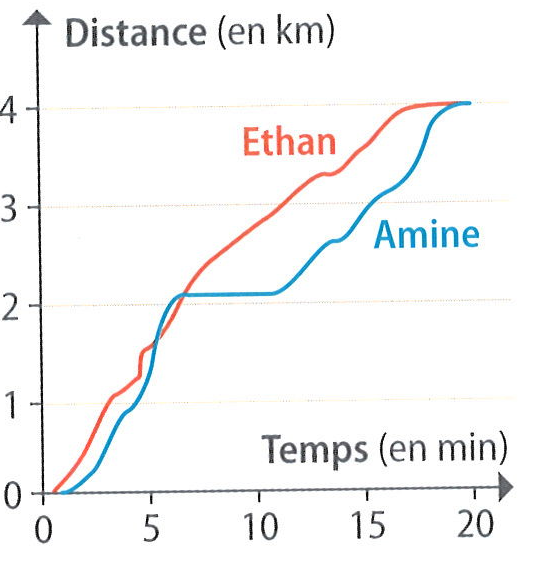
\includegraphics[scale=0.5]{cross}
\end{center}

\begin{questions}
	\question[1] \'Ethan et Amine ont-ils terminé la course ?
	\fillwithdottedlines{3cm}
	
	\question[1] Combien de temps ont-ils couru ?
	\fillwithdottedlines{3cm}
	
	\question[2] Lequel des deux s'est arrêté ? Expliquer la réponse.
	\fillwithdottedlines{4cm}
\end{questions}